\documentclass[conference]{IEEEtran}

\usepackage{graphicx}
\usepackage{amsmath}
\usepackage{listings}
\usepackage{xcolor}
\usepackage{float}

\lstset{
    basicstyle=\ttfamily\footnotesize,
    breaklines=true,
    frame=single,
    columns=fullflexible,
    keepspaces=true,
    showstringspaces=false,
    tabsize=4
}

\begin{document}

\title{Design and Verification of a Basic Single-Cycle RISC-V Processor}

\author{
\IEEEauthorblockN{Abdul Rafay}
\IEEEauthorblockA{
Reg. No. 2024017\\
Ghulam Ishaq Khan Institute of Engineering\\
Sciences and Technology}
\and
\IEEEauthorblockN{Haris Farooq}
\IEEEauthorblockA{
Reg. No. 2024395\\
Ghulam Ishaq Khan Institute of Engineering\\
Sciences and Technology}
}

\maketitle

\begin{abstract}
This report presents the design and verification of a basic single-cycle RISC-V processor implemented in Verilog. The processor supports eight instructions: \texttt{add}, \texttt{sub}, \texttt{and}, \texttt{or}, \texttt{addi}, \texttt{lw}, \texttt{sw}, and \texttt{beq}. The design includes instruction memory, data memory, register file, control unit, immediate generator, ALU control unit, ALU, and program counter update logic. Verification was performed using a Verilog testbench and waveform inspection in GTKWave.
\end{abstract}

\begin{IEEEkeywords}
RISC-V, Verilog, single-cycle processor, ALU, testbench, GTKWave
\end{IEEEkeywords}

\section{Introduction}
The objective of this project was to design a simple single-cycle processor based on a small subset of the RISC-V instruction set. In a single-cycle processor, each instruction completes in one clock cycle. Although this approach is not optimized for performance, it is useful for understanding the basic datapath and control signals of a processor.

The implemented processor supports arithmetic, logical, memory, and branch instructions. The design was tested using a dedicated testbench that stores two values in memory, loads them back, performs ALU operations on the loaded values, and finally checks branch operation using \texttt{beq}.

\section{Supported Instructions}
The processor supports eight instructions, as shown in Table~\ref{tab:instructions}.

\begin{table}[h]
\centering
\caption{Supported Instructions}
\label{tab:instructions}
\begin{tabular}{|c|c|c|}
\hline
\textbf{Instruction} & \textbf{Type} & \textbf{Purpose} \\
\hline
\texttt{add} & R-type & Adds two registers \\
\texttt{sub} & R-type & Subtracts two registers \\
\texttt{and} & R-type & Bitwise AND of two registers \\
\texttt{or} & R-type & Bitwise OR of two registers \\
\texttt{addi} & I-type & Adds register and immediate \\
\texttt{lw} & I-type & Loads word from memory \\
\texttt{sw} & S-type & Stores word to memory \\
\texttt{beq} & B-type & Branches if registers are equal \\
\hline
\end{tabular}
\end{table}

\section{Processor Architecture}
The processor contains the following main components:

\begin{itemize}
    \item Program counter, used to select the current instruction.
    \item Instruction memory, used to store the test program.
    \item Register file, containing 32 registers.
    \item Control unit, used to generate control signals from the opcode.
    \item Immediate generator, used for I-type, S-type, and B-type instructions.
    \item ALU control unit, used to select the ALU operation.
    \item ALU, used for addition, subtraction, AND, OR, and branch comparison.
    \item Data memory, used by \texttt{lw} and \texttt{sw}.
\end{itemize}

The first ALU input is taken from \texttt{read\_data1}. The second ALU input is selected using the \texttt{alu\_src} signal. For R-type and branch instructions, the second input is \texttt{read\_data2}. For \texttt{addi}, \texttt{lw}, and \texttt{sw}, the second input is the immediate value.

\begin{figure}[h]
\centering
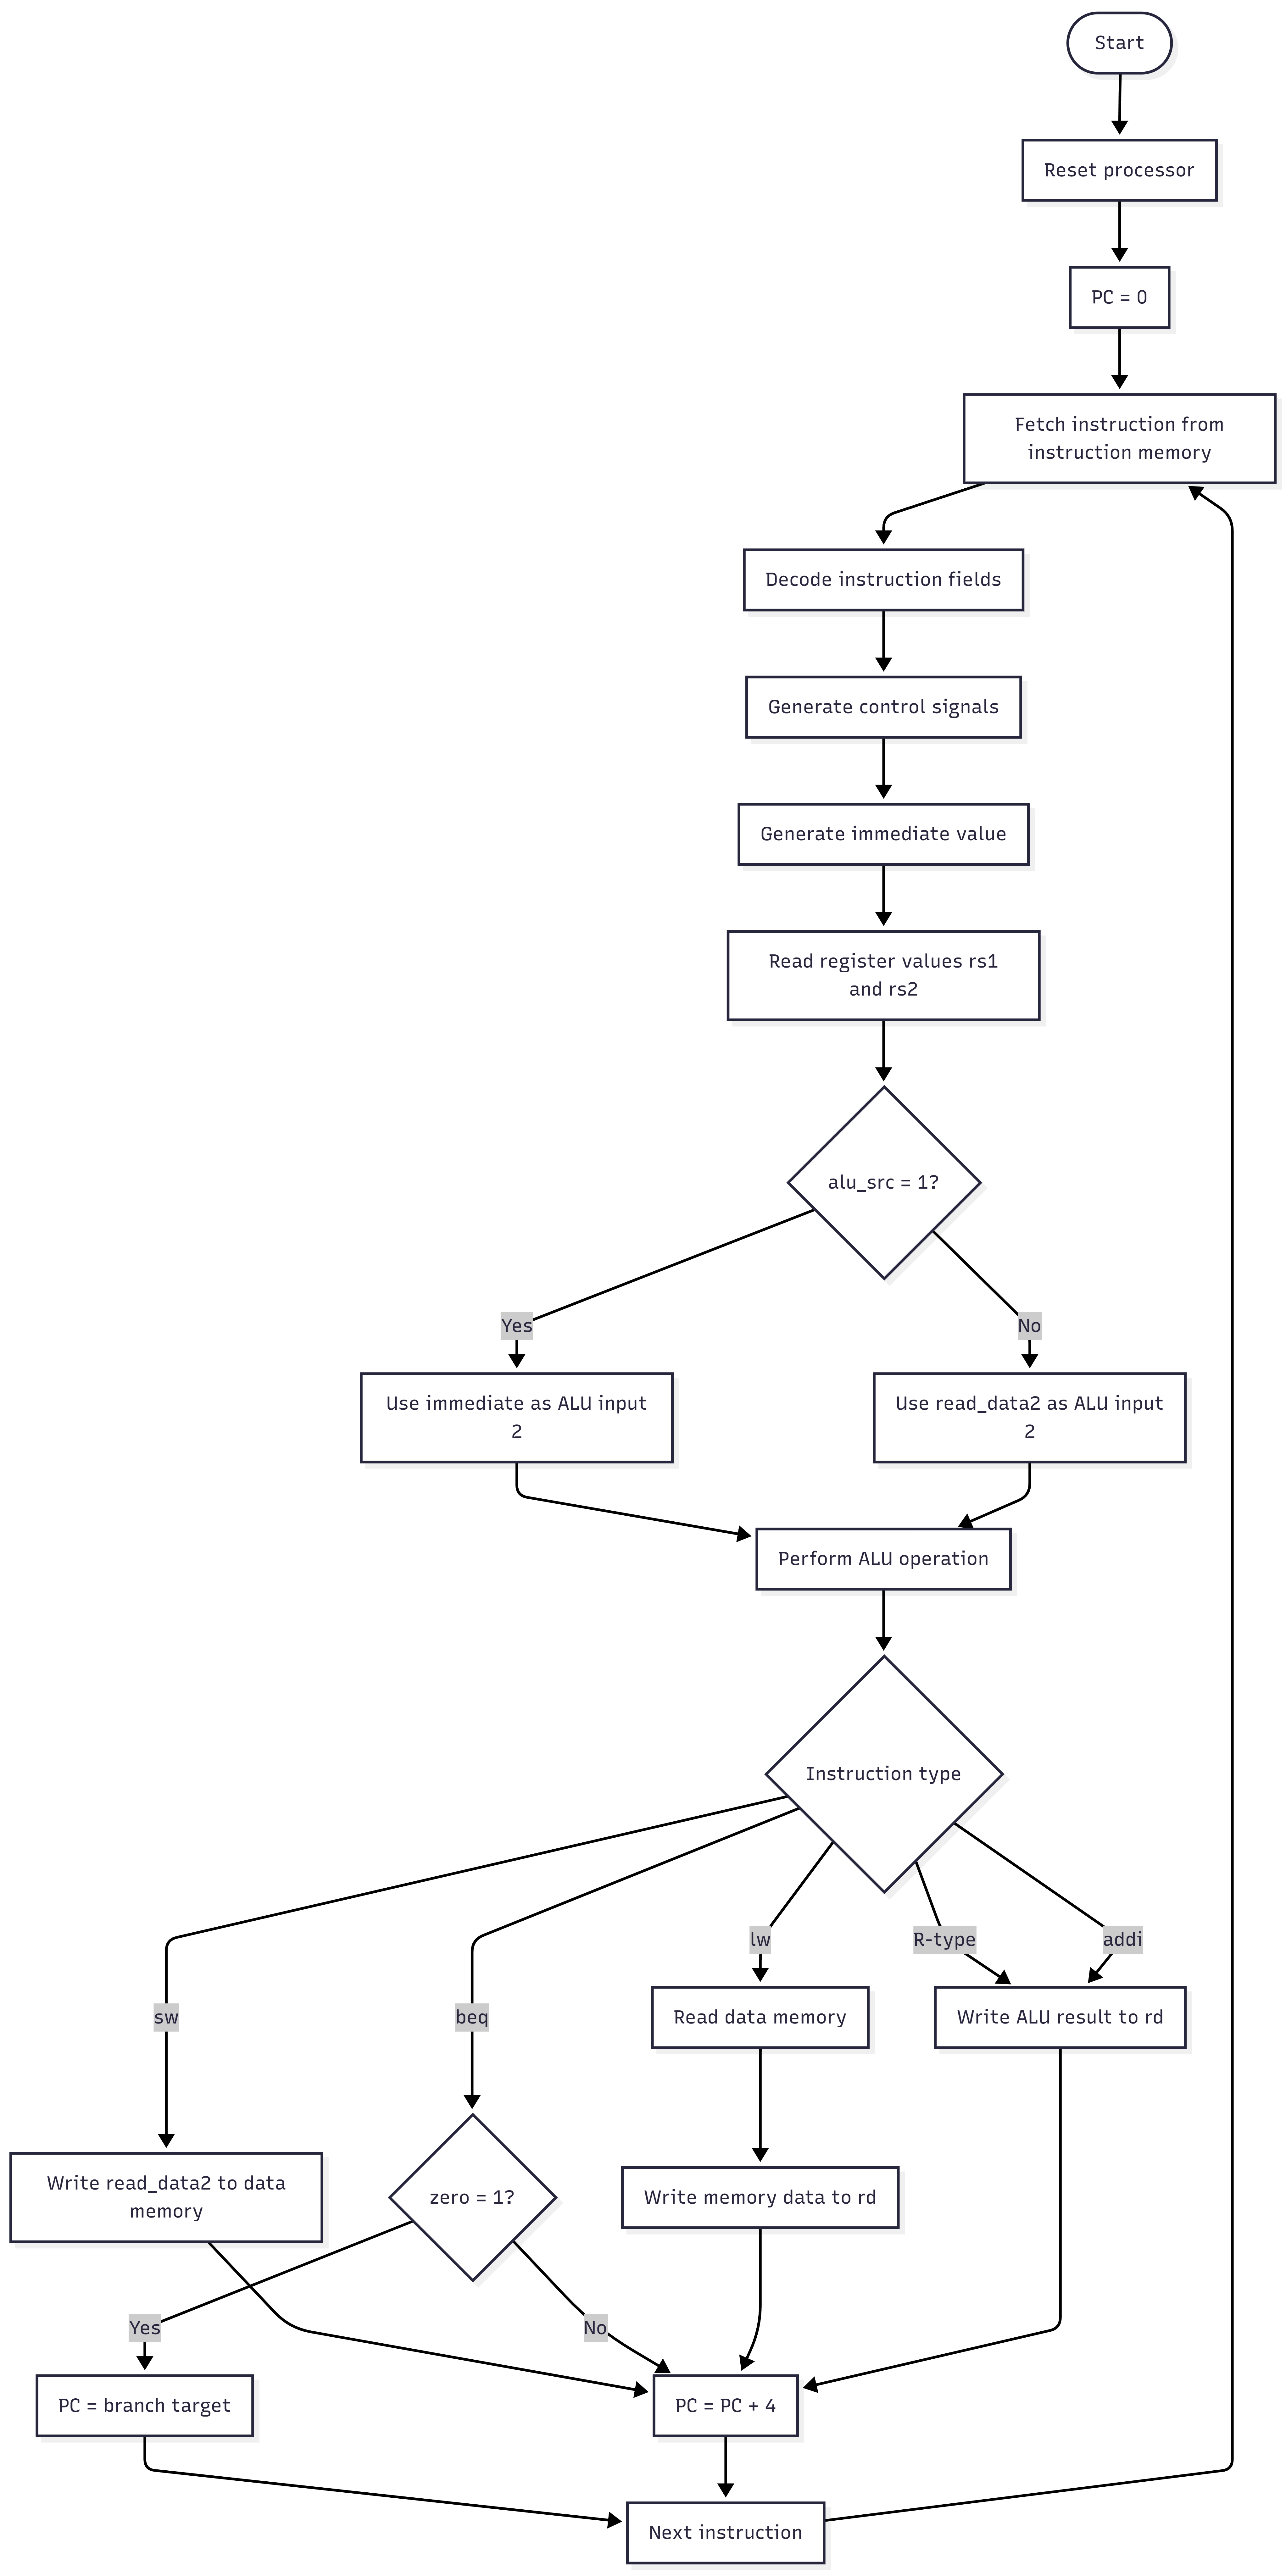
\includegraphics[width=0.48\textwidth]{flowchart.png}
\caption{Flowchart of the single-cycle processor instruction execution process.}
\label{fig:processor_flowchart}
\end{figure}

Fig.~\ref{fig:processor_flowchart} summarizes the instruction flow from reset and instruction fetch to decode, ALU operation, memory access, writeback, and PC update.

\section{Control Signals}
The control unit decodes the opcode and generates the required control signals. The \texttt{alu\_op} signal is used to select the general ALU operation category. The meaning of \texttt{alu\_op} is shown in Table~\ref{tab:aluop}.

\begin{table}[h]
\centering
\caption{ALU Operation Signal}
\label{tab:aluop}
\begin{tabular}{|c|c|c|}
\hline
\textbf{\texttt{alu\_op}} & \textbf{Decimal} & \textbf{Used For} \\
\hline
\texttt{00} & 0 & \texttt{addi}, \texttt{lw}, \texttt{sw} \\
\texttt{01} & 1 & \texttt{beq} \\
\texttt{10} & 2 & R-type instructions \\
\texttt{11} & 3 & Not used \\
\hline
\end{tabular}
\end{table}

The final ALU operation is selected using \texttt{alu\_ctrl}, as shown in Table~\ref{tab:aluctrl}.

\begin{table}[h]
\centering
\caption{ALU Control Signal}
\label{tab:aluctrl}
\begin{tabular}{|c|c|c|}
\hline
\textbf{\texttt{alu\_ctrl}} & \textbf{Decimal} & \textbf{Operation} \\
\hline
\texttt{0000} & 0 & AND \\
\texttt{0001} & 1 & OR \\
\texttt{0010} & 2 & ADD \\
\texttt{0110} & 6 & SUBTRACT \\
\hline
\end{tabular}
\end{table}

\section{Testing Method}
The testbench \texttt{processor\_all\_tb.v} was written to verify all supported instructions. The program first creates two values using \texttt{addi}, stores them in memory using \texttt{sw}, loads them back using \texttt{lw}, and then performs \texttt{add}, \texttt{sub}, \texttt{and}, and \texttt{or} on the loaded values. At the end, \texttt{beq} is tested by skipping one instruction.

The test program performs the following operations:

\begin{lstlisting}
addi x1, x0, 12
addi x2, x0, 5
sw   x1, 0(x0)
sw   x2, 4(x0)
lw   x3, 0(x0)
lw   x4, 4(x0)
add  x5, x3, x4
sub  x6, x3, x4
and  x7, x3, x4
or   x8, x3, x4
beq  x5, x5, 8
addi x9, x0, 99
addi x10, x0, 1
\end{lstlisting}

The instruction \texttt{addi x9, x0, 99} should be skipped because the \texttt{beq} condition is true. Therefore, \texttt{x9} should remain zero.

\section{Simulation Results}
The simulation produced the following expected final values:

\begin{table}[h]
\centering
\caption{Expected Final Register and Memory Values}
\label{tab:results}
\begin{tabular}{|c|c|c|}
\hline
\textbf{Signal} & \textbf{Expected Value} & \textbf{Reason} \\
\hline
\texttt{x1} & 12 & First value \\
\texttt{x2} & 5 & Second value \\
\texttt{x3} & 12 & Loaded from memory[0] \\
\texttt{x4} & 5 & Loaded from memory[1] \\
\texttt{x5} & 17 & \texttt{12 + 5} \\
\texttt{x6} & 7 & \texttt{12 - 5} \\
\texttt{x7} & 4 & \texttt{12 AND 5} \\
\texttt{x8} & 13 & \texttt{12 OR 5} \\
\texttt{x9} & 0 & Skipped by \texttt{beq} \\
\texttt{x10} & 1 & Executed after branch \\
\texttt{memory[0]} & 12 & Stored first value \\
\texttt{memory[1]} & 5 & Stored second value \\
\hline
\end{tabular}
\end{table}

The testbench displayed \texttt{ALL INSTRUCTIONS TEST PASSED}, confirming that all implemented instructions worked correctly.

\section{Waveform Verification}
Waveform verification was performed using GTKWave. The main signals observed were \texttt{pc}, \texttt{instruction}, \texttt{opcode}, \texttt{alu\_op}, \texttt{alu\_ctrl}, \texttt{read\_data1}, \texttt{read\_data2}, \texttt{alu\_input2}, \texttt{alu\_result}, \texttt{reg\_write}, \texttt{mem\_write}, \texttt{mem\_read\_data}, \texttt{branch}, \texttt{zero}, and selected registers. The following waveform screenshots show each instruction in the test program.

Fig.~\ref{fig:addi_x1} shows the first immediate addition. The processor reads \texttt{x0 = 0}, selects the immediate value 12 using \texttt{alu\_src}, computes \texttt{alu\_result = 12}, and writes the result into \texttt{x1}.

\begin{figure}[h]
\centering
\includegraphics[width=0.48\textwidth]{{addi x1,x0,12}.png}
\caption{Waveform for \texttt{addi x1, x0, 12}. The ALU adds \texttt{x0} and immediate value 12, and the result is written to \texttt{x1}.}
\label{fig:addi_x1}
\end{figure}

Fig.~\ref{fig:addi_x2} shows the second immediate addition. The ALU computes \texttt{0 + 5}, and the value 5 is written into \texttt{x2}. These two values are later stored in data memory.

\begin{figure}[h]
\centering
\includegraphics[width=0.48\textwidth]{{addi x2, x0, 5}.png}
\caption{Waveform for \texttt{addi x2, x0, 5}. The immediate value 5 is written to \texttt{x2}.}
\label{fig:addi_x2}
\end{figure}

Fig.~\ref{fig:sw_x1} verifies the first store instruction. Here \texttt{mem\_write = 1}, the calculated address is 0, and the value from \texttt{x1} is written into memory location 0.

\begin{figure}[h]
\centering
\includegraphics[width=0.48\textwidth]{{sw x1, 0(x0)}.png}
\caption{Waveform for \texttt{sw x1, 0(x0)}. The value 12 from \texttt{x1} is stored at memory address 0.}
\label{fig:sw_x1}
\end{figure}

Fig.~\ref{fig:sw_x2} verifies the second store instruction. The ALU calculates address 4, which maps to memory index 1 because the data memory is word addressed using \texttt{alu\_result[7:2]}.

\begin{figure}[h]
\centering
\includegraphics[width=0.48\textwidth]{{sw x2, 4(x0)}.png}
\caption{Waveform for \texttt{sw x2, 4(x0)}. The value 5 from \texttt{x2} is stored at memory address 4, which corresponds to memory index 1.}
\label{fig:sw_x2}
\end{figure}

Fig.~\ref{fig:lw_x3} shows the first load instruction. The processor reads memory address 0, places the memory output on \texttt{mem\_read\_data}, and writes the loaded value 12 into \texttt{x3}.

\begin{figure}[h]
\centering
\includegraphics[width=0.48\textwidth]{{lw x3, 0(x0)}.png}
\caption{Waveform for \texttt{lw x3, 0(x0)}. The value 12 is loaded from memory address 0 and written to \texttt{x3}.}
\label{fig:lw_x3}
\end{figure}

Fig.~\ref{fig:lw_x4} shows the second load instruction. The address 4 selects memory index 1, so the value 5 is loaded and written into \texttt{x4}.

\begin{figure}[h]
\centering
\includegraphics[width=0.48\textwidth]{{lw x4, 4(x0)}.png}
\caption{Waveform for \texttt{lw x4, 4(x0)}. The value 5 is loaded from memory address 4 and written to \texttt{x4}.}
\label{fig:lw_x4}
\end{figure}

Fig.~\ref{fig:add_x5} verifies the R-type add instruction. The ALU takes the loaded values from \texttt{x3} and \texttt{x4}, computes \texttt{12 + 5 = 17}, and writes the result to \texttt{x5}.

\begin{figure}[h]
\centering
\includegraphics[width=0.48\textwidth]{{add x5, x3, x4}.png}
\caption{Waveform for \texttt{add x5, x3, x4}. The loaded values 12 and 5 are added, giving \texttt{x5 = 17}.}
\label{fig:add_x5}
\end{figure}

Fig.~\ref{fig:sub_x6} verifies subtraction. The ALU control signal selects subtract operation, so the processor computes \texttt{12 - 5 = 7} and stores the result in \texttt{x6}.

\begin{figure}[h]
\centering
\includegraphics[width=0.48\textwidth]{{sub x6, x3, x4}.png}
\caption{Waveform for \texttt{sub x6, x3, x4}. The loaded values are subtracted, giving \texttt{x6 = 7}.}
\label{fig:sub_x6}
\end{figure}

Fig.~\ref{fig:and_x7} verifies the bitwise AND operation. With \texttt{alu\_ctrl = 0}, the ALU computes \texttt{12 AND 5 = 4}, and the result is written into \texttt{x7}.

\begin{figure}[h]
\centering
\includegraphics[width=0.48\textwidth]{{and x7, x3, x4}.png}
\caption{Waveform for \texttt{and x7, x3, x4}. The bitwise AND of 12 and 5 gives \texttt{x7 = 4}.}
\label{fig:and_x7}
\end{figure}

Fig.~\ref{fig:or_x8} verifies the bitwise OR operation. With \texttt{alu\_ctrl = 1}, the ALU computes \texttt{12 OR 5 = 13}, and the result is written into \texttt{x8}.

\begin{figure}[h]
\centering
\includegraphics[width=0.48\textwidth]{{or x8, x3, x4}.png}
\caption{Waveform for \texttt{or x8, x3, x4}. The bitwise OR of 12 and 5 gives \texttt{x8 = 13}.}
\label{fig:or_x8}
\end{figure}

Fig.~\ref{fig:beq} verifies the branch instruction. Since \texttt{x5} is compared with itself, the ALU subtraction gives zero, \texttt{zero = 1}, and \texttt{pc\_src = 1}. Therefore, the next PC jumps over the instruction that would write 99 into \texttt{x9}.

\begin{figure}[h]
\centering
\includegraphics[width=0.48\textwidth]{{beq x5, x5, 8}.png}
\caption{Waveform for \texttt{beq x5, x5, 8}. Since both operands are equal, \texttt{zero = 1}, \texttt{pc\_src = 1}, and the next PC skips the instruction that would write 99 to \texttt{x9}.}
\label{fig:beq}
\end{figure}

\section{Conclusion}
A basic single-cycle RISC-V processor was implemented and verified in Verilog. The processor supports eight instructions: \texttt{add}, \texttt{sub}, \texttt{and}, \texttt{or}, \texttt{addi}, \texttt{lw}, \texttt{sw}, and \texttt{beq}. The testbench verifies the complete instruction set by storing values in memory, loading them back, performing ALU operations, and checking branch behavior. Simulation and waveform inspection confirm that the processor works as expected.

\appendices

\section{Processor Verilog Code}
The complete processor source code is included below.

\begin{lstlisting}[caption={Complete processor.v source code},label={lst:processor}]
`timescale 1ns/1ps

// Basic single cycle RISC-V processor
// Instructions supported: add, sub, and, or, addi, lw, sw, beq

module processor(
    input clk,
    input reset
);
    // Main storage used by the processor
    reg [31:0] pc;
    reg [31:0] instr_mem [0:63];
    reg [31:0] data_mem  [0:63];
    reg [31:0] regs      [0:31];

    // Instruction fields
    wire [31:0] instruction;
    wire [6:0] opcode;
    wire [4:0] rd;
    wire [2:0] funct3;
    wire [4:0] rs1;
    wire [4:0] rs2;
    wire [6:0] funct7;

    wire branch;
    wire mem_read;
    wire mem_to_reg;
    wire [1:0] alu_op;
    wire mem_write;
    wire alu_src;
    wire reg_write;

    wire [31:0] read_data1;
    wire [31:0] read_data2;
    wire [31:0] imm;
    wire [3:0] alu_ctrl;
    wire [31:0] alu_input2;
    wire [31:0] alu_result;
    wire zero;
    wire [31:0] mem_read_data;
    wire [31:0] write_data;

    wire [31:0] pc_plus_4;
    wire [31:0] branch_target;
    wire pc_src;
    wire [31:0] next_pc;

    integer i;

    // pc is a byte address, so pc[7:2] gives the instruction word index
    assign instruction = instr_mem[pc[7:2]];

    assign opcode = instruction[6:0];
    assign rd     = instruction[11:7];
    assign funct3 = instruction[14:12];
    assign rs1    = instruction[19:15];
    assign rs2    = instruction[24:20];
    assign funct7 = instruction[31:25];

    control_unit control(
        .opcode(opcode),
        .branch(branch),
        .mem_read(mem_read),
        .mem_to_reg(mem_to_reg),
        .alu_op(alu_op),
        .mem_write(mem_write),
        .alu_src(alu_src),
        .reg_write(reg_write)
    );

    imm_gen immediate_generator(
        .instruction(instruction),
        .imm(imm)
    );

    alu_control alu_control_unit(
        .alu_op(alu_op),
        .funct3(funct3),
        .funct7(funct7),
        .alu_ctrl(alu_ctrl)
    );

    // Register x0 is always zero
    assign read_data1 = (rs1 == 0) ? 32'b0 : regs[rs1];
    assign read_data2 = (rs2 == 0) ? 32'b0 : regs[rs2];

    assign alu_input2 = alu_src ? imm : read_data2;

    alu main_alu(
        .a(read_data1),
        .b(alu_input2),
        .alu_ctrl(alu_ctrl),
        .result(alu_result),
        .zero(zero)
    );

    assign mem_read_data = data_mem[alu_result[7:2]];
    assign write_data = mem_to_reg ? mem_read_data : alu_result;

    assign pc_plus_4 = pc + 4;
    assign branch_target = pc + imm;
    assign pc_src = branch & zero;
    assign next_pc = pc_src ? branch_target : pc_plus_4;

    always @(posedge clk or posedge reset) begin
        if (reset) begin
            pc <= 0;
            for (i = 0; i < 32; i = i + 1)
                regs[i] <= 0;
            for (i = 0; i < 64; i = i + 1)
                data_mem[i] <= 0;
        end else begin
            pc <= next_pc;

            if (mem_write)
                data_mem[alu_result[7:2]] <= read_data2;

            if (reg_write && rd != 0)
                regs[rd] <= write_data;
        end
    end
endmodule

module control_unit(
    input [6:0] opcode,
    output reg branch,
    output reg mem_read,
    output reg mem_to_reg,
    output reg [1:0] alu_op,
    output reg mem_write,
    output reg alu_src,
    output reg reg_write
);
    always @(*) begin
        // Default values
        branch = 0;
        mem_read = 0;
        mem_to_reg = 0;
        alu_op = 2'b00;
        mem_write = 0;
        alu_src = 0;
        reg_write = 0;

        case (opcode)
            7'b0110011: begin // add, sub, and, or
                alu_op = 2'b10;
                reg_write = 1;
            end
            7'b0010011: begin // addi
                alu_op = 2'b00;
                alu_src = 1;
                reg_write = 1;
            end
            7'b0000011: begin // lw
                mem_read = 1;
                mem_to_reg = 1;
                alu_src = 1;
                reg_write = 1;
            end
            7'b0100011: begin // sw
                alu_src = 1;
                mem_write = 1;
            end
            7'b1100011: begin // beq
                branch = 1;
                alu_op = 2'b01;
            end
        endcase
    end
endmodule

module imm_gen(
    input [31:0] instruction,
    output reg [31:0] imm
);
    wire [6:0] opcode;
    assign opcode = instruction[6:0];

    always @(*) begin
        case (opcode)
            7'b0010011,
            7'b0000011:
                imm = {{20{instruction[31]}}, instruction[31:20]};

            7'b0100011:
                imm = {{20{instruction[31]}}, instruction[31:25], instruction[11:7]};

            7'b1100011:
                imm = {{19{instruction[31]}}, instruction[31], instruction[7],
                       instruction[30:25], instruction[11:8], 1'b0};

            default:
                imm = 32'b0;
        endcase
    end
endmodule

module alu_control(
    input [1:0] alu_op,
    input [2:0] funct3,
    input [6:0] funct7,
    output reg [3:0] alu_ctrl
);
    always @(*) begin
        case (alu_op)
            2'b00:
                alu_ctrl = 4'b0010; // add for lw, sw, addi
            2'b01:
                alu_ctrl = 4'b0110; // subtract for beq
            2'b10: begin
                case ({funct7, funct3})
                    10'b0000000_000: alu_ctrl = 4'b0010; // add
                    10'b0100000_000: alu_ctrl = 4'b0110; // sub
                    10'b0000000_111: alu_ctrl = 4'b0000; // and
                    10'b0000000_110: alu_ctrl = 4'b0001; // or
                    default:         alu_ctrl = 4'b0010;
                endcase
            end
            default:
                alu_ctrl = 4'b0010;
        endcase
    end
endmodule

module alu(
    input [31:0] a,
    input [31:0] b,
    input [3:0] alu_ctrl,
    output reg [31:0] result,
    output zero
);
    always @(*) begin
        case (alu_ctrl)
            4'b0000: result = a & b;
            4'b0001: result = a | b;
            4'b0010: result = a + b;
            4'b0110: result = a - b;
            default: result = 0;
        endcase
    end

    assign zero = (result == 0);
endmodule
\end{lstlisting}

\section{Testbench Verilog Code}
The complete all-instruction testbench source code is included below.

\begin{lstlisting}[caption={Complete processor_all_tb.v source code},label={lst:testbench}]
`timescale 1ns/1ps

module processor_all_tb;
    reg clk;
    reg reset;

    // Extra signals for easy viewing in GTKWave
    wire [31:0] x1;
    wire [31:0] x2;
    wire [31:0] x3;
    wire [31:0] x4;
    wire [31:0] x5;
    wire [31:0] x6;
    wire [31:0] x7;
    wire [31:0] x8;
    wire [31:0] x9;
    wire [31:0] x10;
    wire [31:0] mem0;
    wire [31:0] mem1;

    processor uut(
        .clk(clk),
        .reset(reset)
    );

    assign x1 = uut.regs[1];
    assign x2 = uut.regs[2];
    assign x3 = uut.regs[3];
    assign x4 = uut.regs[4];
    assign x5 = uut.regs[5];
    assign x6 = uut.regs[6];
    assign x7 = uut.regs[7];
    assign x8 = uut.regs[8];
    assign x9 = uut.regs[9];
    assign x10 = uut.regs[10];
    assign mem0 = uut.data_mem[0];
    assign mem1 = uut.data_mem[1];

    always #5 clk = ~clk;

    initial begin
        $dumpfile("processor_all_tb.vcd");
        $dumpvars(0, processor_all_tb);

        clk = 0;
        reset = 1;

        // Program:
        // Store two values in memory, load them back,
        // then use the loaded values for add, sub, and, or.
        uut.instr_mem[0]  = 32'h00C00093; // addi x1, x0, 12
        uut.instr_mem[1]  = 32'h00500113; // addi x2, x0, 5
        uut.instr_mem[2]  = 32'h00102023; // sw   x1, 0(x0)
        uut.instr_mem[3]  = 32'h00202223; // sw   x2, 4(x0)
        uut.instr_mem[4]  = 32'h00002183; // lw   x3, 0(x0)
        uut.instr_mem[5]  = 32'h00402203; // lw   x4, 4(x0)
        uut.instr_mem[6]  = 32'h004182B3; // add  x5, x3, x4
        uut.instr_mem[7]  = 32'h40418333; // sub  x6, x3, x4
        uut.instr_mem[8]  = 32'h0041F3B3; // and  x7, x3, x4
        uut.instr_mem[9]  = 32'h0041E433; // or   x8, x3, x4
        uut.instr_mem[10] = 32'h00528463; // beq  x5, x5, 8
        uut.instr_mem[11] = 32'h06300493; // addi x9, x0, 99 (should skip)
        uut.instr_mem[12] = 32'h00100513; // addi x10, x0, 1

        #12;
        reset = 0;

        #180;

        $display("x1 = %0d", uut.regs[1]);
        $display("x2 = %0d", uut.regs[2]);
        $display("x3 = %0d", uut.regs[3]);
        $display("x4 = %0d", uut.regs[4]);
        $display("x5 = %0d", uut.regs[5]);
        $display("x6 = %0d", uut.regs[6]);
        $display("x7 = %0d", uut.regs[7]);
        $display("x8 = %0d", uut.regs[8]);
        $display("x9 = %0d", uut.regs[9]);
        $display("x10 = %0d", uut.regs[10]);
        $display("memory[0] = %0d", uut.data_mem[0]);
        $display("memory[1] = %0d", uut.data_mem[1]);

        if (uut.regs[1] == 12 &&
            uut.regs[2] == 5 &&
            uut.regs[3] == 12 &&
            uut.regs[4] == 5 &&
            uut.regs[5] == 17 &&
            uut.regs[6] == 7 &&
            uut.regs[7] == 4 &&
            uut.regs[8] == 13 &&
            uut.regs[9] == 0 &&
            uut.regs[10] == 1 &&
            uut.data_mem[0] == 12 &&
            uut.data_mem[1] == 5)
            $display("ALL INSTRUCTIONS TEST PASSED");
        else
            $display("ALL INSTRUCTIONS TEST FAILED");

        $finish;
    end
endmodule
\end{lstlisting}

\end{document}
